\documentclass[c_worksheet.tex]{subfiles}

\begin{document}
  
\chapter{Files - Input - Output}
In C meint das Wort \textit{File} nicht eine Datei auf der Festplatte sondern etwas Anderes. Ein File ist ein Objekt, das sich im \textit{lesenden} Modus oder im \textit{schreibeden} Modus befinden kann. In ein File, das gerade im Modus \textit{schreibend} ist, kann man Daten hineinstecken. Aus einem File, das gerade im \textit{lesenden} Modus ist, kann man Daten heraus nehmen. Ob hinter dem File eine Datei auf der Festplatte oder einem USB-Stick, ein Stück Speicher, ein Kabel zu einem anderen Rechner oder etwas ganz Anderes steckt, macht für den Programmierer keinen Unterschied. Alle diese Dinge sind für den Programmierer nur ein Objekt vom Typ \textit{File}. In \textbf{stdio.h} findet man Funktionen um Files zu öffnen und zu schließen, Daten zu lesen und zu schreiben.\\
Wenn ein neues Programm gestartet wird, dann hat es von Anfang an schon 3 geöffnete Files, die bei Programmende automisch geschlossen werden. \textbf{stdin}, \textbf{stdout} und \textbf{stderr}

\begin{figure}[h]
\centering
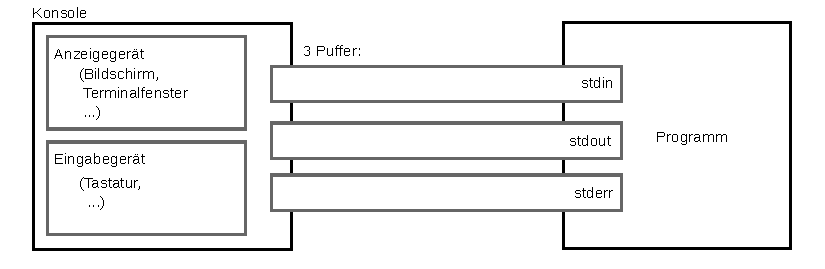
\includegraphics[width=0.8\textwidth]{./Grafiken/Files/stdFiles}
\end{figure}

\textbf{stdin} befindet sich immer im lesenden Modus. In dieses File werden automatisch die Symbole gelegt, die der Benutzer auf der Tastatur drückt. Die Funktion \textit{scanf} arbeitet auf diesem File.

\begin{figure}[h]
\centering
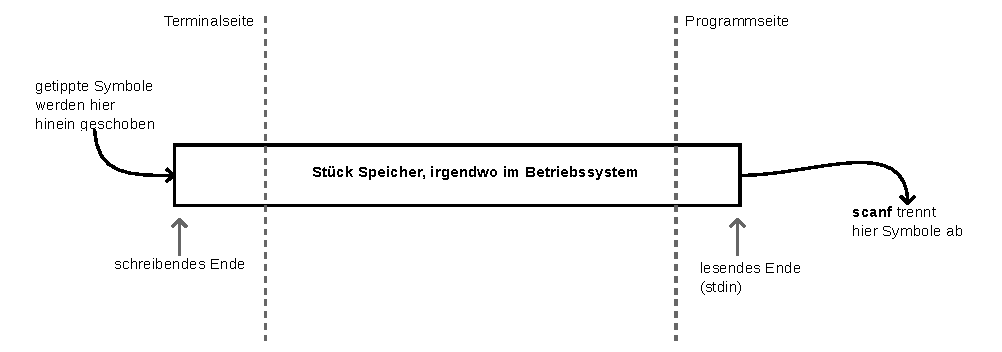
\includegraphics[width=0.9\textwidth]{./Grafiken/Files/stdin}
\end{figure}

\textbf{stdout} befindet sich im schreibenden Modus. Symbole, die man mit der Funktion \textit{printf} in stdout hinein gibt, werden auf dem Bildschirm angezeigt.\\
\textbf{stderr} befindet sich auch im schreibenden Modus und kann meistens genau so wie stdin benutzt werden. Das File stderr ist dafür gedacht Errormeldungen auszugeben, während stdout für den \textit{normalen} Output vorgesehen ist. Die meisten Terminals werden die Symbole, die man in stdout und stderr hinein gibt gleichermaßen auf dem Bildschirm anzeigen. Aber es gibt auch Terminals, die die Symbole von stderr hervorheben (z.B. rot und fett darstellen) oder in einer Logdatei auf der Festplatte abspeichern.

\section{IO Funktionen}

\textbf{printf} und \textbf{scanf} arbeiten auf den Files stdout und stdin. Die Funktionen \textbf{fprintf} und \textbf{fscanf} funktionieren genauso, aber nehmen als zusätzlichen Parameter noch das File mit dem gearbeitet werden soll.

\begin{lstlisting}[numbers=none]
printf("Ich gehe an stdout\n");
fprintf(stdout, "Ich auch\n");
fprintf(stderr, "Ich bin eine Fehlermeldung\n");
\end{lstlisting}

Mit der Funktion \textbf{fopen} kann man ein neues File öffnen, das zu einer \textit{echten} Datei auf der Festplatte zeigt. Dafür muss man den Dateipfad und den Modus angeben. Die einfachsten Modi sind dabei \textbf{"r"} (read) und \textbf{"w"} (write). Mit der Funktion \textbf{fclose} kann das File wieder geschlossen werden.

\begin{lstlisting}
#include <stdio.h>

int main(void) {
    FILE * in  = fopen("./AusgangsDatei.txt", "r");
    FILE * out = fopen("./ZielDatei.txt", "w");
    int i;

    fscanf(in, "%d", &i);
    fprintf(out, "In der AusgangsDatei stand die Zahl: %d", i);

    fclose(in);
    fclose(out);
    return 0;
}
\end{lstlisting}

\begin{lstlisting}
#include <stdio.h>

int main(void) {
    FILE * log = ("./logDatei", "w");
    int i;
    
    fscanf(stdin, "%d", &i);
    fprintf(log, "Der Benutzer hat die Zahl: %d ", i);
    fprintf(log, "auf der Konsole eingetippt");

    fclose(log);
    return 0;
}
\end{lstlisting}


\end{document}